%\documentclass[10pt,journal,letterpaper,compsoc]{IEEEtran}
\documentclass[10pt, journal, letterpaper]{article}
\usepackage[utf8]{inputenc}

\usepackage[backend=bibtex, style=numeric, sorting=none]{biblatex}
%\nocite{*} -- Include all reference, even if not cited in the text

\usepackage{comment}

% Format and Images
\usepackage{graphicx}
% Spacing %
%\usepackage{float}
\usepackage{xspace}
% Code %
\usepackage{verbatim}
\usepackage{listings}
\lstset{basicstyle=\footnotesize, frame=single}

% References and links
%\usepackage{cleveref} %for reference auto capitalization (cref, Cref)
%\usepackage{acronym} %manage acronyms
\usepackage{url}
%\usepackage{hyperref} %hyper reference in pdf % include as last package

%%% Customizations %%%
% Change linespacing for itemize:
\let\olditemize\itemize
\renewcommand\itemize{\olditemize\setlength\itemsep{1pt}\parskip0pt}
%%% Change linespacing for enumerate:
\let\oldenumerate\enumerate
\renewcommand\enumerate{\oldenumerate\setlength\itemsep{1pt}\parskip0pt}

% Fix default hyphenation when splitting word to new line
%\hyphenation{a-na-ly-sis a-va-i-la-bi-li-ty dis-tin-gui-sha-ble i-ma-ges}

%%% Custom Commands %%%
%   \hide : comment text within other text
\newcommand{\hide}[1]{}

%%%%%%%%%%%%%%%%%%%%%%%%%%%%%%%%%%%%%%%%%%%%%%%%%%%%%%%%%%%%%%%%%%%%%%%%%%%%%%
\usepackage{lipsum}

\newcommand{\solname}{XYZ\xspace}

\title{\solname: Research Paper Template}
\author{Name Surname, Name Surname}

\addbibresource{bibliography}
	
\begin{document}
	\maketitle
		
	\begin{abstract}
	\lipsum[1-2]
	\end{abstract}
	
	\section{Introduction}
	\label{sect:intro}
	Cite foundation papers\cite{lamport1994latex}.
	\lipsum[3-4]
	
	\subsection{Motivation}
	\label{sect:motivation}
	\lipsum[5-6]
	
	\section{\solname: Project description}\label{sect:project}
	This section describes \solname.
	
	\subsection{Goals}
	\label{sect:goals}
	\lipsum[9]

	\subsection{Approach}
	\label{sect:approach}
	\lipsum[10]
		
	%%%%% Design %%%%%
	\section{Design}
	\label{sect:design}
	\lipsum[11]

	%%%%% Architecture %%%%%
	\section{Architecture}
	The HyBIS architecture is shown in Figure \ref{fig:frz-arch}.
	
	\begin{figure}
		\centering
		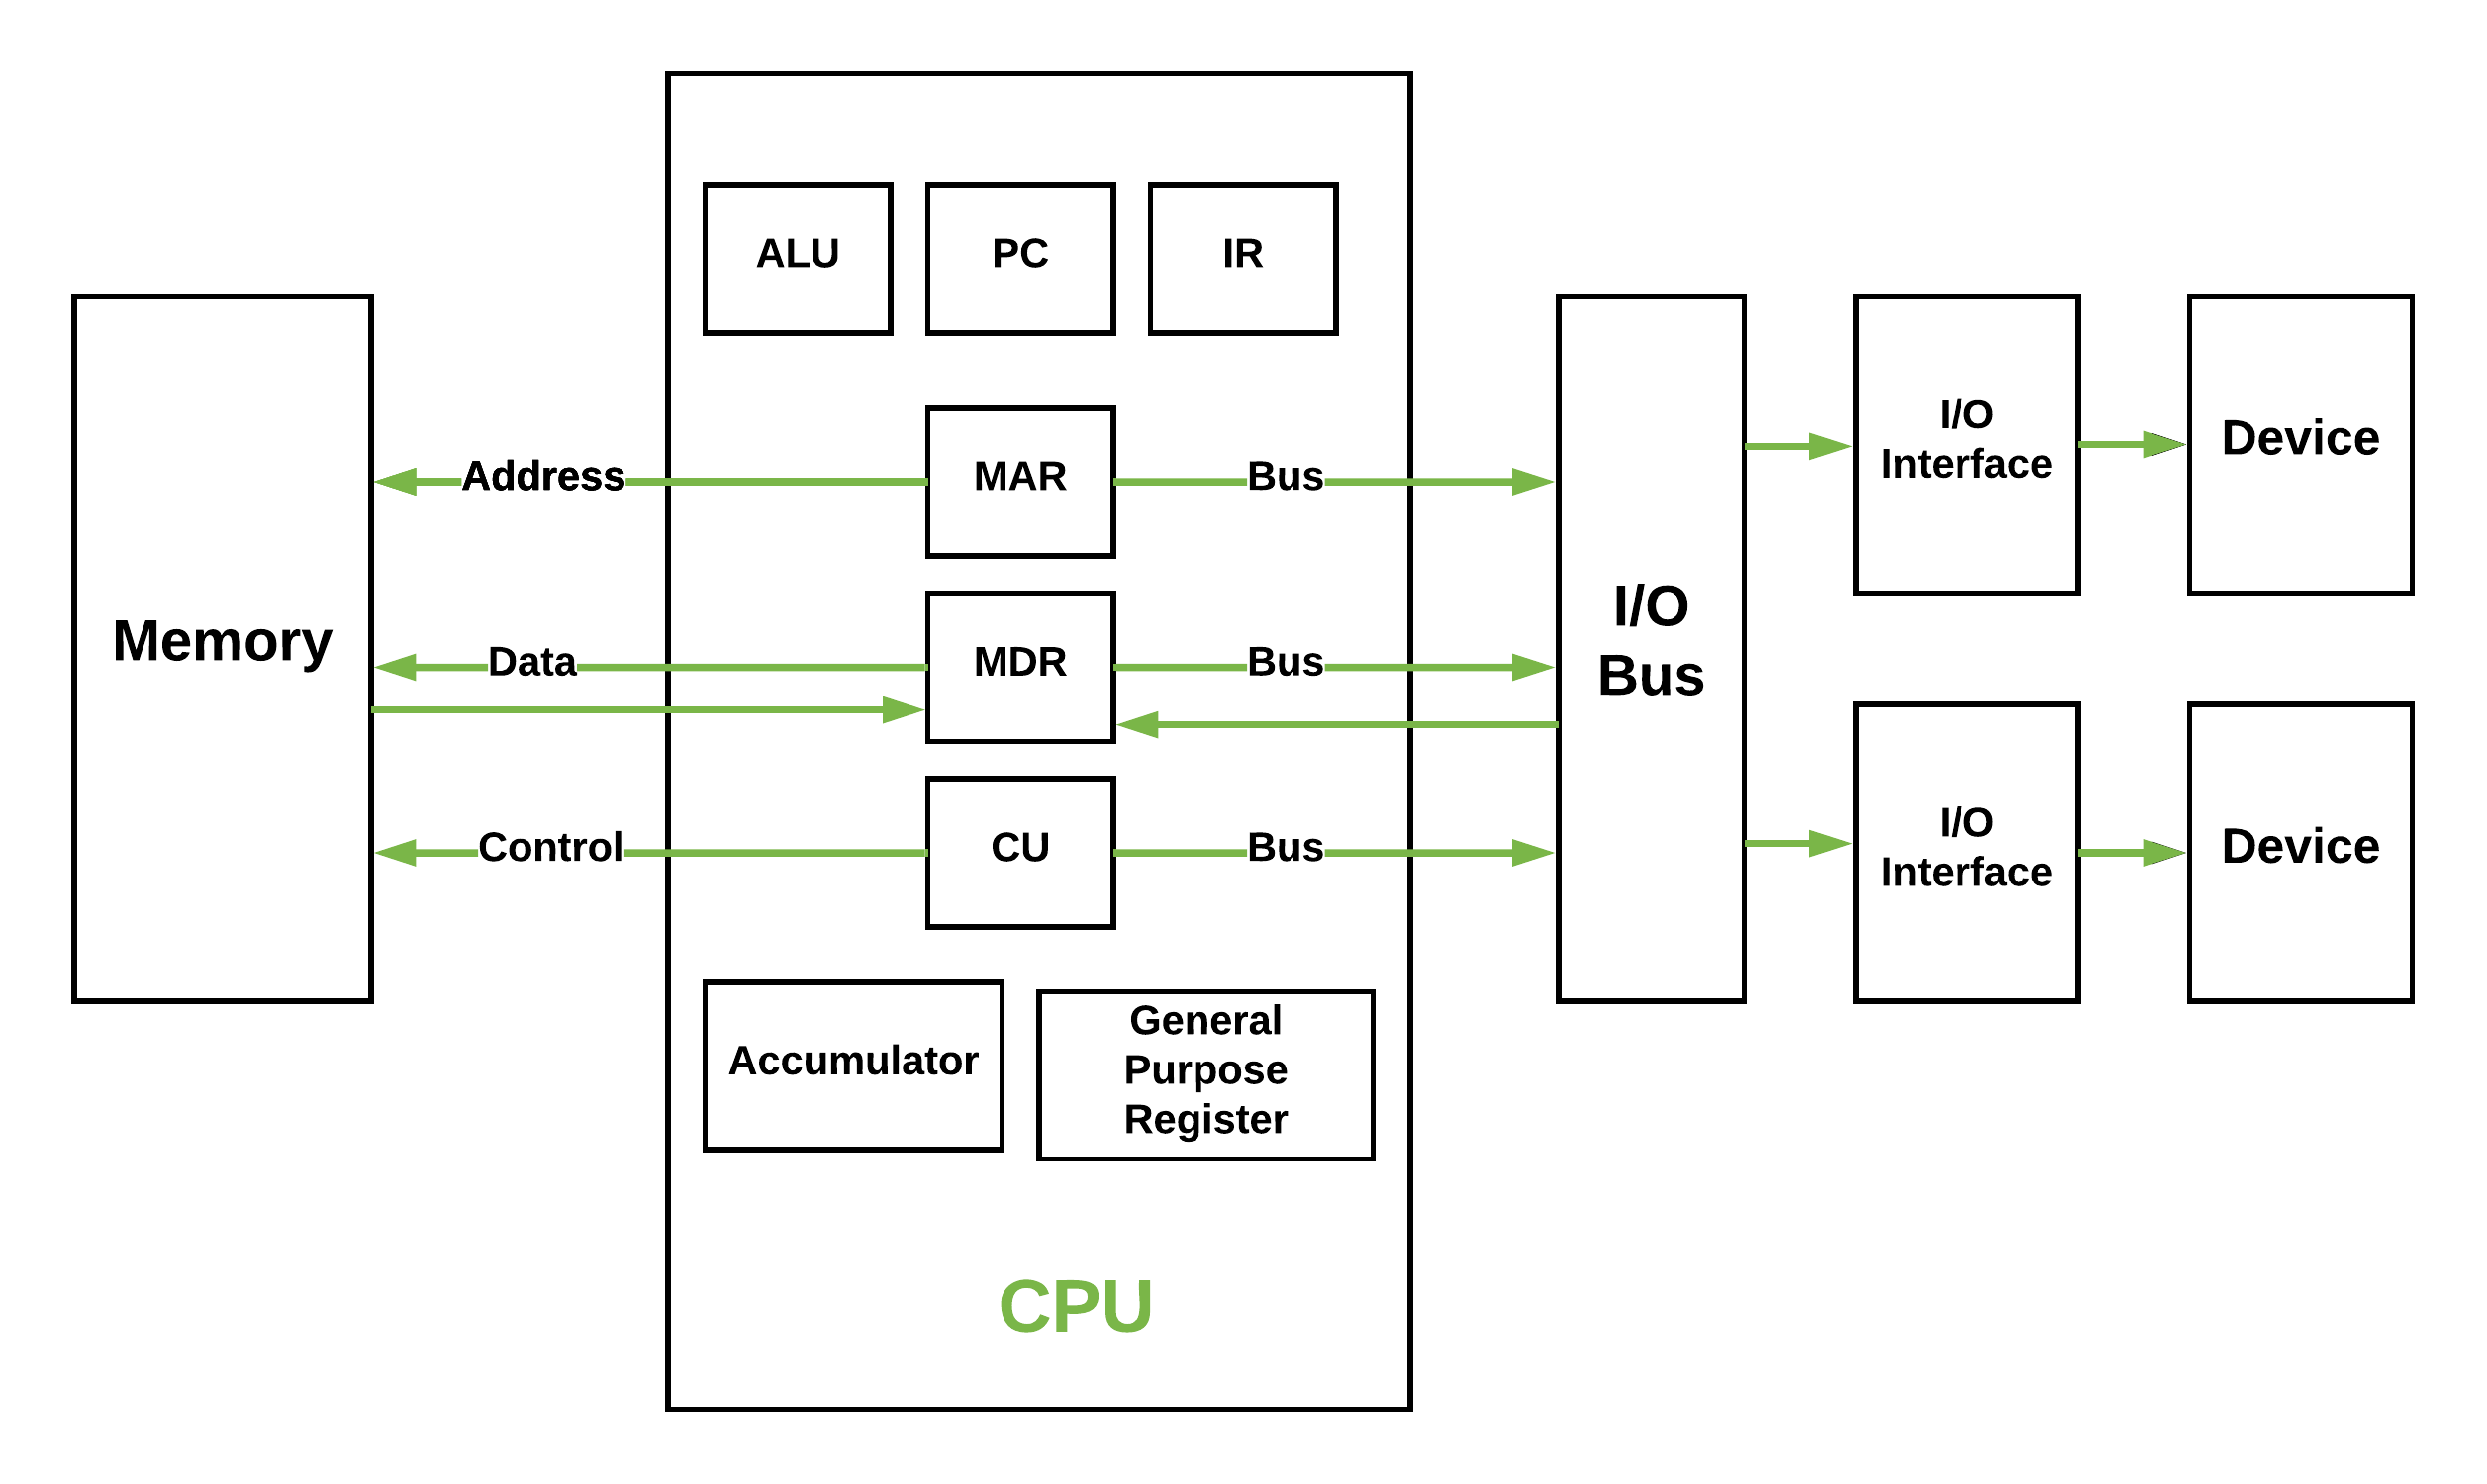
\includegraphics[width=\columnwidth]{img/computer-architecture} 
		\caption{\solname Architecture}
		\label{fig:frz-arch}
	\end{figure}
	\lipsum[12]
	
	\subsection{\solname Components:}
	\lipsum[13]

	%%%%% Implementation %%%%%
	\section{Implementation}
	\lipsum[14]
	
	%Technologies
	\subsection{Technology Details}
	\lipsum[15]

	%%%%% Evaluation %%%%%
	\section{Evaluation}
	\lipsum[16-17]
	
	%%%%% Discussion %%%%%
	\section{Discussion}
	\lipsum[18]
	\subsection{Contribution}
	\lipsum[7-8]
	
	%%%%% Related Work %%%%%
	\section{Related Work}
	Cite related articles\cite{day1998write}.
	\lipsum[19]

	%%%%% Conclusion %%%%%
	\section{Conclusion and Future Work}
	\label{conclusion}
	\lipsum[19]

	\printbibliography
%\bibliographystyle{ieeetr}
%\bibliography{bibliography}	
\end{document}
